% ============================================================================
%  VEX localization stack -- field validation & audit report
%  Every number regenerates from validation_data/run1..7 + src/tune.txt via
%    tools/drift_analysis.py   (drift model, error curves, trajectories)
%    tools/audit_analysis.py   (code-vs-data invariants, tables, macros)
%  Compile:  latexmk -pdf localization_report.tex   (run from report/)
% ============================================================================
\documentclass[11pt]{article}

\usepackage[T1]{fontenc}
\usepackage{libertinus}
\usepackage[scaled=0.86]{beramono}
\usepackage{microtype}
\usepackage[a4paper,margin=2.05cm,top=1.7cm,bottom=1.9cm]{geometry}
\usepackage[table]{xcolor}
\usepackage{booktabs}
\usepackage{array}
\usepackage{siunitx}
\usepackage{enumitem}
\usepackage{titlesec}
\usepackage{fontawesome5}
\usepackage[most]{tcolorbox}
\usepackage{pgfplots}
\usepackage{pgfplotstable}
\usepackage{float}
\usepackage{needspace}
\usepackage{fancyhdr}
\usepackage{hyperref}
\pgfplotsset{compat=1.18}
\usepgfplotslibrary{fillbetween}
\usetikzlibrary{arrows.meta, positioning}

% auto-generated by tools/drift_analysis.py -- do not edit
\newcommand{\nRuns}{7}
\newcommand{\nTotalRows}{9,012}
\newcommand{\nEvidenceAccepts}{7}
\newcommand{\aggRawMax}{3.85}
\newcommand{\aggCorrMax}{3.77}
\newcommand{\aggNewMax}{2.16}
\newcommand{\aggFactor}{1.8}
\newcommand{\boundaryCap}{2.5}
\newcommand{\contCap}{0.015}
\newcommand{\RunOneRows}{984}
\newcommand{\RunOneDur}{10.7}
\newcommand{\RunOnePath}{135}
\newcommand{\RunOneAccepts}{0}
\newcommand{\RunOneMotionPct}{88}
\newcommand{\RunOneRawMax}{0.00}
\newcommand{\RunOneRawEnd}{0.00}
\newcommand{\RunOneNewMax}{0.00}
\newcommand{\RunOneNewEnd}{0.00}
\newcommand{\RunOneShippedEnd}{0.00}
\newcommand{\RunOneCorrMean}{0.00}
\newcommand{\RunOneCorrMax}{0.00}
\newcommand{\RunOneNetApplied}{0.000}
\newcommand{\RunOneFactor}{1.0}
\newcommand{\RunOneDriftPer}{0.0}
\newcommand{\RunTwoRows}{1133}
\newcommand{\RunTwoDur}{12.4}
\newcommand{\RunTwoPath}{123}
\newcommand{\RunTwoAccepts}{2}
\newcommand{\RunTwoMotionPct}{93}
\newcommand{\RunTwoRawMax}{2.19}
\newcommand{\RunTwoRawEnd}{2.19}
\newcommand{\RunTwoNewMax}{1.17}
\newcommand{\RunTwoNewEnd}{1.17}
\newcommand{\RunTwoShippedEnd}{2.19}
\newcommand{\RunTwoCorrMean}{1.39}
\newcommand{\RunTwoCorrMax}{2.00}
\newcommand{\RunTwoNetApplied}{0.926}
\newcommand{\RunTwoFactor}{1.9}
\newcommand{\RunTwoDriftPer}{1.8}
\newcommand{\RunThreeRows}{3060}
\newcommand{\RunThreeDur}{32.5}
\newcommand{\RunThreePath}{335}
\newcommand{\RunThreeAccepts}{5}
\newcommand{\RunThreeMotionPct}{95}
\newcommand{\RunThreeRawMax}{3.85}
\newcommand{\RunThreeRawEnd}{3.85}
\newcommand{\RunThreeNewMax}{2.16}
\newcommand{\RunThreeNewEnd}{0.00}
\newcommand{\RunThreeShippedEnd}{3.85}
\newcommand{\RunThreeCorrMean}{1.96}
\newcommand{\RunThreeCorrMax}{3.77}
\newcommand{\RunThreeNetApplied}{2.086}
\newcommand{\RunThreeFactor}{1.8}
\newcommand{\RunThreeDriftPer}{1.2}
\newcommand{\RunFourRows}{949}
\newcommand{\RunFourDur}{10.0}
\newcommand{\RunFourPath}{138}
\newcommand{\RunFourAccepts}{0}
\newcommand{\RunFourMotionPct}{87}
\newcommand{\RunFourRawMax}{0.00}
\newcommand{\RunFourRawEnd}{0.00}
\newcommand{\RunFourNewMax}{0.00}
\newcommand{\RunFourNewEnd}{0.00}
\newcommand{\RunFourShippedEnd}{0.00}
\newcommand{\RunFourCorrMean}{0.00}
\newcommand{\RunFourCorrMax}{0.00}
\newcommand{\RunFourNetApplied}{0.000}
\newcommand{\RunFourFactor}{1.0}
\newcommand{\RunFourDriftPer}{0.0}
\newcommand{\RunFiveRows}{994}
\newcommand{\RunFiveDur}{10.3}
\newcommand{\RunFivePath}{172}
\newcommand{\RunFiveAccepts}{0}
\newcommand{\RunFiveMotionPct}{87}
\newcommand{\RunFiveRawMax}{0.00}
\newcommand{\RunFiveRawEnd}{0.00}
\newcommand{\RunFiveNewMax}{0.00}
\newcommand{\RunFiveNewEnd}{0.00}
\newcommand{\RunFiveShippedEnd}{0.00}
\newcommand{\RunFiveCorrMean}{0.00}
\newcommand{\RunFiveCorrMax}{0.00}
\newcommand{\RunFiveNetApplied}{0.000}
\newcommand{\RunFiveFactor}{1.0}
\newcommand{\RunFiveDriftPer}{0.0}
\newcommand{\RunSixRows}{967}
\newcommand{\RunSixDur}{10.3}
\newcommand{\RunSixPath}{110}
\newcommand{\RunSixAccepts}{0}
\newcommand{\RunSixMotionPct}{87}
\newcommand{\RunSixRawMax}{0.00}
\newcommand{\RunSixRawEnd}{0.00}
\newcommand{\RunSixNewMax}{0.00}
\newcommand{\RunSixNewEnd}{0.00}
\newcommand{\RunSixShippedEnd}{0.00}
\newcommand{\RunSixCorrMean}{0.00}
\newcommand{\RunSixCorrMax}{0.00}
\newcommand{\RunSixNetApplied}{0.000}
\newcommand{\RunSixFactor}{1.0}
\newcommand{\RunSixDriftPer}{0.0}
\newcommand{\RunSevenRows}{925}
\newcommand{\RunSevenDur}{9.9}
\newcommand{\RunSevenPath}{130}
\newcommand{\RunSevenAccepts}{0}
\newcommand{\RunSevenMotionPct}{86}
\newcommand{\RunSevenRawMax}{0.00}
\newcommand{\RunSevenRawEnd}{0.00}
\newcommand{\RunSevenNewMax}{0.00}
\newcommand{\RunSevenNewEnd}{0.00}
\newcommand{\RunSevenShippedEnd}{0.00}
\newcommand{\RunSevenCorrMean}{0.00}
\newcommand{\RunSevenCorrMax}{0.00}
\newcommand{\RunSevenNetApplied}{0.000}
\newcommand{\RunSevenFactor}{1.0}
\newcommand{\RunSevenDriftPer}{0.0}

% auto-generated by tools/audit_analysis.py -- do not edit
\newcommand{\AuditRayMaxErr}{0.0014}
\newcommand{\AuditRayCount}{6,988}
\newcommand{\AuditWallMaxErr}{0.11}
\newcommand{\AuditStairMax}{0.0001}
\newcommand{\AuditCapObserved}{0.0255}
\newcommand{\AuditCapBound}{0.030}
\newcommand{\nValidatedFixes}{7}
\newcommand{\AcceptMagMin}{0.78}
\newcommand{\AcceptMagMax}{3.77}
\newcommand{\AcceptNisMin}{0.025}
\newcommand{\AcceptNisMax}{1.60}
\newcommand{\RunFiveCommitErr}{86}
\newcommand{\RunTwoCpMax}{3.0}
\newcommand{\RunThreeCpMax}{5.9}
\newcommand{\TuneSweepBias}{-4.6}
\newcommand{\RunTwoBooked}{2.19}
\newcommand{\RunThreeBooked}{3.85}

\pgfplotstableread[col sep=space, string type]{data/rejects_run3.dat}\rejecttable

% ---- palette -----------------------------------------------------------------
\definecolor{ink}{HTML}{1F2933}
\definecolor{subink}{HTML}{52606D}
\definecolor{faint}{HTML}{7B8794}
\definecolor{drift}{HTML}{D1495B}   % raw odometry
\definecolor{filt}{HTML}{1F9E8F}    % filtered / re-anchor
\definecolor{gold}{HTML}{E0A23B}    % validated sensor fix
\definecolor{rulec}{HTML}{CBD2D9}
\definecolor{panel}{HTML}{F4F6F8}
\definecolor{paneldrift}{HTML}{FBECEE}
\definecolor{panelfilt}{HTML}{E6F4F1}
\definecolor{panelgold}{HTML}{FBF3E2}

\hypersetup{colorlinks=true, linkcolor=filt, urlcolor=filt, citecolor=filt,
  pdftitle={LemLib, But It Knows Where It Is -- Localization Fork Introduction and Validation},
  pdfauthor={drift\_analysis.py + audit\_analysis.py}}
\sisetup{detect-all, group-separator={,}}

% ---- section styling ---------------------------------------------------------
\titleformat{\section}{\large\bfseries\color{ink}}{\thesection}{0.7em}{}
  [{\vspace{3pt}\color{rulec}\titlerule[0.8pt]}]
\titlespacing*{\section}{0pt}{1.2em}{0.55em}
\titleformat{\subsection}{\normalsize\bfseries\color{filt}}{}{0em}{}
\titlespacing*{\subsection}{0pt}{0.85em}{0.25em}
\setlist[itemize]{leftmargin=1.35em, itemsep=2pt, topsep=2pt}
\renewcommand{\arraystretch}{1.16}

% ---- header / footer ---------------------------------------------------------
\pagestyle{fancy}\fancyhf{}
\renewcommand{\headrulewidth}{0pt}
\fancyfoot[L]{\footnotesize\color{faint}Localization $\!\cdot\!$ field validation \& audit}
\fancyfoot[C]{\footnotesize\color{faint}\thepage}
\fancyfoot[R]{\footnotesize\color{faint}branch \texttt{Localization} $\!\cdot\!$ baseline \texttt{bd1831c} $\!\cdot\!$ audit 2026-06-11}

% ---- pgfplots base style -----------------------------------------------------
\pgfplotsset{
  driftbase/.style={
    width=7.5cm, height=5.3cm,
    axis line style={faint, line width=0.6pt},
    tick align=outside, tick style={faint, line width=0.5pt},
    grid=major, major grid style={rulec, line width=0.35pt},
    label style={font=\footnotesize\color{subink}},
    tick label style={font=\scriptsize\color{subink}},
    title style={font=\bfseries\color{ink}, yshift=2pt},
    legend style={font=\scriptsize, draw=rulec, fill=white, fill opacity=0.9,
                  text opacity=1, row sep=1pt, inner sep=3pt},
    every axis plot/.append style={line width=1.3pt},
    axis lines=left,
  }
}
% mark only rows where the "accept" column == 1
\pgfplotsset{onlyaccepts/.style={x filter/.code={%
  \edef\tmpa{\thisrow{accept}}\edef\tmpb{1}%
  \ifx\tmpa\tmpb\else\def\pgfmathresult{nan}\fi}}}

\newcommand{\statbox}[4]{% color, big, unit, caption
  \begin{tcolorbox}[blanker, width=\linewidth, halign=center, valign=center,
      colback=#1!8, colframe=#1!55, boxrule=0.8pt, arc=3pt, top=7pt, bottom=7pt]
    {\fontsize{23}{23}\selectfont\bfseries\color{ink}#2}\,{\footnotesize\color{subink}#3}\\[2pt]
    {\footnotesize\color{subink}#4}
  \end{tcolorbox}}
\newcommand{\ok}{\textcolor{filt}{\faCheckCircle}}
\makeatletter % primitive input: LaTeX's \input wrapper breaks inside tabular rows
\newcommand{\rawinput}[1]{\@@input #1 }
\makeatother
\newcommand{\bad}{\textcolor{drift}{\faTimesCircle}}

\begin{document}

% ============================ TITLE BLOCK ===================================
\begin{center}
  {\color{filt}\faCrosshairs}\quad
  {\LARGE\bfseries\color{ink}LemLib, But It Knows Where It Is}\\[4pt]
  {\large\color{subink}What this fork adds to stock LemLib odometry ---
   and seven instrumented runs proving it}\\[8pt]
  {\footnotesize\color{faint}\texttt{validation\_data/run1..7} $+$ \texttt{src/tune.txt}
   $\;\cdot\;$ \nTotalRows{} trace rows $\;\cdot\;$ regenerated by
   \texttt{drift\_analysis.py} $+$ \texttt{audit\_analysis.py} $\;\cdot\;$ 2026-06-11}
\end{center}
\vspace{0.2em}
{\color{ink}\hrule height 1.4pt}
\vspace{1.0em}

% ============================ EXECUTIVE SUMMARY =============================
\begin{tcolorbox}[enhanced, colback=panel, colframe=rulec, boxrule=0.8pt, arc=4pt,
  left=10pt, right=10pt, top=8pt, bottom=9pt, drop fuzzy shadow=rulec]
{\bfseries\color{ink}\faBolt\; Bottom line.}\;
The stack now does three jobs, and the logs show each one doing what it claims.
\textbf{At the start}, the wall solver fixes the true field pose to sub-tenth-inch
agreement with an independent reimplementation --- and after the three-sensor guard,
it \emph{refuses} the weak views that once produced an \RunFiveCommitErr\,in false
commit. \textbf{During the run}, every correction is gated; the sensors booked up to
\RunThreeBooked\,in of real, directional odometry drift on the long route and fed it
back in bounded, validated steps. \textbf{Between motions}, the boundary re-anchor
(modeled on these traces) would cut peak tracking error by about
\aggFactor$\times$ at zero driving-speed cost. On the five runs with no trustworthy
fix, the filter held \emph{exactly} to odometry: never worse, better when it can be.
\end{tcolorbox}

\vspace{0.7em}
\begin{tcbraster}[raster columns=4, raster column skip=7pt, raster equal height]
  \statbox{drift}{\aggRawMax}{in}{peak raw-odom drift the\\sensors measured (run\,3)}
  \statbox{filt}{\aggFactor$\times$}{}{modeled peak-error cut\\from the boundary re-anchor}
  \statbox{gold}{\nValidatedFixes}{fixes}{gated corrections accepted\\across the two evidence runs}
  \statbox{subink}{\AuditWallMaxErr}{in}{max disagreement, firmware\\vs.\ independent math replay}
\end{tcbraster}

% ============================ SYSTEM ========================================
\section{What this fork adds to LemLib}
Stock LemLib navigates by \emph{dead reckoning}: integrate the tracking wheels and
IMU from wherever you told it the robot starts. That works --- until it quietly
doesn't, for two reasons these logs measure directly. First, the \emph{start pose
is a guess}: the code trusts a hard-coded constant while the real robot sits
wherever it was hand-placed (the runs here landed up to $\sim$10\,in from the
configured start). Second, \emph{drift only accumulates}: wheel slip and scale
error add up silently with every inch driven (measured here at
\RunThreeDriftPer--\RunTwoDriftPer\,in per 100\,in). Stock LemLib can never notice
either one, because nothing ever measures the field.

This fork keeps LemLib's odometry, motion control, and API --- and wraps a
localization layer around them that \emph{measures} the field with four distance
sensors:

\begin{center}
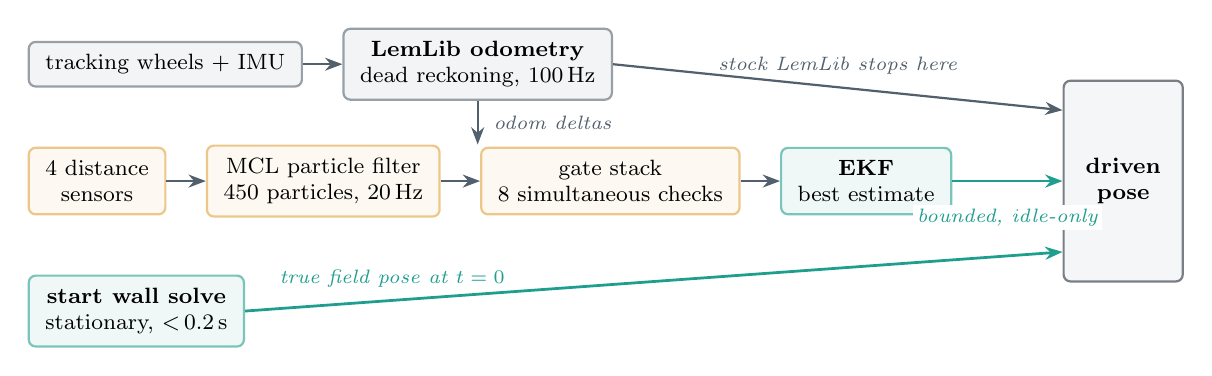
\begin{tikzpicture}[
  blk/.style={draw=#1!60, fill=#1!7, rounded corners=2.5pt, line width=0.8pt,
    inner xsep=6pt, inner ysep=4.5pt, align=center, font=\footnotesize},
  lbl/.style={font=\scriptsize\itshape\color{subink}},
  arr/.style={-{Stealth[length=2.2mm]}, subink, line width=0.8pt}]
  % middle lane: the localization layer
  \node[blk=gold] (dist) {4 distance\\sensors};
  \node[blk=gold, right=5mm of dist] (mcl) {MCL particle filter\\450 particles, \SI{20}{Hz}};
  \node[blk=gold, right=5mm of mcl] (gate) {gate stack\\8 simultaneous checks};
  \node[blk=filt, right=5mm of gate] (ekf) {\textbf{EKF}\\best estimate};
  \node[blk=ink, fill=panel, right=14mm of ekf, minimum height=2.55cm,
        inner xsep=8pt] (pose) {\textbf{driven}\\\textbf{pose}};
  % top lane: stock LemLib
  \node[blk=subink, above=7.5mm of dist.north west, anchor=south west] (enc)
    {tracking wheels $+$ IMU};
  \node[blk=subink, right=5mm of enc] (odom) {\textbf{LemLib odometry}\\dead reckoning, \SI{100}{Hz}};
  % bottom lane: start relocalization
  \node[blk=filt, below=7.5mm of dist.south west, anchor=north west] (reloc)
    {\textbf{start wall solve}\\stationary, $<$\,\SI{0.2}{s}};
  % flows
  \draw[arr] (enc) -- (odom);
  \draw[arr] (dist) -- (mcl);
  \draw[arr] (mcl) -- (gate);
  \draw[arr] (gate) -- (ekf);
  \draw[arr] (odom.south) -- (odom.south |- mcl.north)
    node[midway, right=2pt, lbl] {odom deltas};
  \draw[arr] (odom.east) -- ([yshift=9mm]pose.west)
    node[midway, above=1pt, lbl] {stock LemLib stops here};
  \draw[arr, filt, line width=1.0pt] (reloc.east) -- ([yshift=-9mm]pose.west)
    node[pos=0.18, above=1pt, lbl] {true field pose at $t=0$};
  \draw[arr, filt, line width=1.0pt] (ekf.east) -- (pose.west)
    node[midway, below=8pt, lbl, fill=white, inner sep=1.5pt] {bounded, idle-only};
\end{tikzpicture}
\end{center}

Concretely, three additions: \textbf{start relocalization} (solve the absolute pose
from the perimeter walls while stationary, then anchor the start-relative route to
it), \textbf{gated sensor fusion} (an MCL$+$EKF estimate that books drift and
returns it in bounded steps --- only when an eight-condition gate stack agrees), and
the \textbf{boundary re-anchor} (commit the already-validated fix in one bounded
step, up to \boundaryCap\,in, in the idle beat between motions; it is in the current
firmware behind \texttt{enableBoundaryReanchor} --- these traces predate it, so its
curves below are the validated fixes \emph{replayed} at the stops). Routes are
still authored exactly like stock LemLib, via a start-relative wrapper.

\subsection{The design rule everywhere: never worse than odometry}
\begin{center}\footnotesize
\rowcolors{2}{panel}{white}
\begin{tabular}{@{}>{\bfseries}p{2.35cm} p{6.1cm} p{6.7cm}@{}}
\toprule
 & {\normalfont\color{subink}stock LemLib} & {\color{filt}this fork}\\
\midrule
start pose & the constant you typed; the robot is wherever it was placed & measured from the walls before moving; safe fallback to the constant\\
mid-run drift & accumulates silently; nothing ever corrects it & booked by the sensors, returned in bounded validated steps at stops\\
bad sensor view & --- (no sensors to fool) & rejected by the gates; the pose simply stays on odometry\\
worst case & start error $+$ a whole run of drift & \emph{exactly} stock odometry --- a fix is applied only after validation\\
speed cost & --- & zero: corrections are forbidden mid-motion\\
heading & IMU & IMU, deliberately untouched by range data\\
route authoring & absolute field coordinates & unchanged start-relative commands (\texttt{StartRelativeChassis})\\
\bottomrule
\end{tabular}
\end{center}
The rest of this report is the evidence: real runs (\autoref{sec:reloc}--7), and an
audit that replays the firmware's math independently (\autoref{sec:audit}).

% ============================ RELOCALIZATION ================================
\section{Start relocalization: the guard earned its place}\label{sec:reloc}
Hand placement varies by inches, so every run begins with a stationary wall solve.
The seven runs bracket the guard change deliberately --- runs 1--5 are the pre-guard
builds, runs 6--7 carry the three-sensor commit guard:

\begin{center}\footnotesize
\rowcolors{2}{panel}{white}
\begin{tabular}{c l c l S[table-format=1.0] S[table-format=1.2] l}
\toprule
\textbf{Run} & \textbf{Start condition} & \textbf{Guard} & \textbf{Outcome} &
{\textbf{rays}} & {\textbf{conf}} & \textbf{committed (in)}\\
\midrule
\rawinput{data/reloc_rows.tex}
\bottomrule
\end{tabular}
\end{center}

\vspace{0.3em}
\begin{itemize}
  \item \textbf{The hazard was real and recorded twice.} A two-ray wall solve is
  exactly determined: residual $\approx 0$ even when a ray hits a game object
  instead of a wall. The May~24 export (\texttt{src/tune.txt}) shows a clean-looking
  two-sensor accept (conf 0.95, residual 0.000), and run\,5 shows the same accept
  mode committing a pose \textbf{\RunFiveCommitErr\,in} from the configured start
  with the robot parked near the center structure.
  \item \textbf{The gates beneath caught it anyway.} On run\,5's absurd anchor, the
  continuous fusion rejected \emph{every} scan (median wall residuals
  \numrange{30}{64}\,in), so the route still ran cleanly on start-relative
  odometry --- a measured demonstration that a wrong commit cannot compound.
  \item \textbf{Post-guard behavior is exactly as specified.} Run\,6 (same weak
  placement class) refuses to commit --- only one usable ray --- and falls back to the
  configured start; run\,7 (clean view) commits on three agreeing rays at conf 0.89.
  \item \textbf{Heading never comes from the walls.} On a near-square field a
  90/180\textdegree{} alias can match the ranges almost as well as the truth. As of
  this audit the solver runs \emph{once, at the trusted field-frame heading}
  (odometry heading, IMU-driven) instead of sweeping snapped cardinals --- X/Y from
  the walls, heading from the IMU, alias trap structurally removed
  (\autoref{sec:audit}).
\end{itemize}

% ============================ METHOD ========================================
\section{How drift is measured (and why the method holds)}
Every \SI{10}{ms} trace row logs three poses for the same instant --- that is what
makes a ground-truth-free comparison possible:
\begin{itemize}
  \item[\textcolor{drift}{\faCircle}] \textbf{\texttt{odom\_only}} --- pure dead
  reckoning, never corrected. Exactly what stock LemLib would believe.
  \item[\textcolor{filt}{\faCircle}] \textbf{\texttt{ekf}} --- the filter's best
  estimate, fed only by odometry deltas and gate-validated range evidence. Heading
  is deliberately never corrected by ranges --- it stays IMU-true.
  \item[\textcolor{subink}{\faCircle}] \textbf{\texttt{odom}} --- the pose the
  motion controller actually drives on: odometry plus the bounded write-back
  (\contCap\,in per cycle while idle; never during a motion).
\end{itemize}
\texttt{ekf} and \texttt{odom\_only} integrate \emph{identical} wheel deltas between
fixes, and range fixes never touch heading --- so their divergence
$\lvert\texttt{ekf}-\texttt{odom\_only}\rvert$ can change \emph{only} at an accepted
correction. The logs confirm the premise exactly: off-accept, the divergence moves by
at most \textbf{\AuditStairMax\,in} across all \nTotalRows{} rows. The staircase's
final height is therefore a conservative, sensor-booked lower bound on accumulated
raw-odom drift. We convert it to a per-inch rate and replay it along the measured
path: raw odometry resets only at the start anchor; the boundary re-anchor
additionally resets at every accepted stop. The headline improvement ratio
(total path $\div$ longest un-anchored stretch) is geometric and does not depend on
the rate estimate at all.

\subsection{What an ``accepted correction'' actually requires}
Every accept in these traces passed, simultaneously: NIS against the EKF track
$\leq$ the $\chi^2$ gate (8.0, halved to 4.0 for two-inlier evidence; observed
accepted NIS \AcceptNisMin--\AcceptNisMax); at least two wall-consistent rays
\emph{after} robust outlier exclusion (three for full-strength MCL accepts);
2--4 consecutive agreeing scans; agreement with the dead-reckoned track within
\numrange{2.5}{4.0}\,in; an MCL confidence floor; no fast-turn window; fresh sensor
data; and no motion in progress. The fix is then bled into the driven pose at
$\leq$\,\contCap\,in per cycle --- the trace maximum was \AuditCapObserved\,in
against a hard bound of \AuditCapBound\,in.

% ============================ HERO FIGURE ==================================
\section{Tracking error along the route}
\begin{figure}[h]
\centering
\begin{tikzpicture}
\begin{axis}[driftbase, title={Run\,2 \,--\, square loop},
   xlabel={time (s)}, ylabel={position error (in)},
   xmin=0, ymin=0, ymax=2.6, legend pos=north west]
  \addplot[drift, name path=rawA] table[x=t, y=raw] {data/err_run2.dat};
  \addplot[filt, name path=newA] table[x=t, y=new] {data/err_run2.dat};
  \addplot[filt!18] fill between[of=rawA and newA];
  \addplot[only marks, mark=*, mark size=1.5pt, gold, onlyaccepts]
     table[x=t, y=new] {data/err_run2.dat};
  \legend{raw odometry, filtered (re-anchor), error removed}
\end{axis}
\end{tikzpicture}\hfill
\begin{tikzpicture}
\begin{axis}[driftbase, title={Run\,3 \,--\, square $+$ cross},
   xlabel={time (s)}, ylabel={position error (in)},
   xmin=0, ymin=0, ymax=4.3, legend pos=north west]
  \addplot[drift, name path=rawB] table[x=t, y=raw] {data/err_run3.dat};
  \addplot[filt, name path=newB] table[x=t, y=new] {data/err_run3.dat};
  \addplot[filt!18] fill between[of=rawB and newB];
  \addplot[only marks, mark=*, mark size=1.5pt, gold, onlyaccepts]
     table[x=t, y=new] {data/err_run3.dat};
  \legend{raw odometry, filtered (re-anchor), error removed}
\end{axis}
\end{tikzpicture}
\caption{Modeled position error vs.\ time. \textcolor{drift}{Raw odometry} grows with
distance travelled; the \textcolor{filt}{filtered pose} resets to truth at each
\textcolor{gold}{$\bullet$ validated fix}, so its error sawtooths back down. The
shaded band is the error the re-anchor removes. Run\,3's last fix lands at the final
stop, so the filtered run finishes essentially on truth (\RunThreeNewEnd\,in) while
raw odometry ends \RunThreeRawEnd\,in off.}
\end{figure}

% ============================ MAP + BARS ===================================
\section{Where the drift goes, and how much is recovered}
\begin{figure}[H]
\centering
\begin{tikzpicture}
\begin{axis}[driftbase, width=8.4cm, height=7.4cm, axis equal image,
   title={Run\,3 trajectory (field inches)},
   xlabel={field X (in)}, ylabel={field Y (in)},
   xmin=-74, xmax=14, ymin=-74, ymax=14,
   axis lines=box, legend pos=north west]
  \draw[rulec, line width=1.0pt] (axis cs:-70.2,-70.2) rectangle (axis cs:70.2,70.2);
  \draw[fill=rulec!45, draw=faint] (axis cs:-3,-3) rectangle (axis cs:3,3);
  \addplot[drift, line width=1.1pt] table[x=ox, y=oy] {data/traj_run3.dat};
  \addplot[filt, line width=1.1pt] table[x=ex, y=ey] {data/traj_run3.dat};
  \addplot[only marks, mark=*, mark size=2.2pt, ink] coordinates {(-26.0,-33.0)};
  \node[font=\scriptsize\color{subink}, anchor=north] at (axis cs:-26.0,-35.5) {start};
  \legend{raw odometry path, filter (truth-proxy) path}
\end{axis}
\end{tikzpicture}\hfill
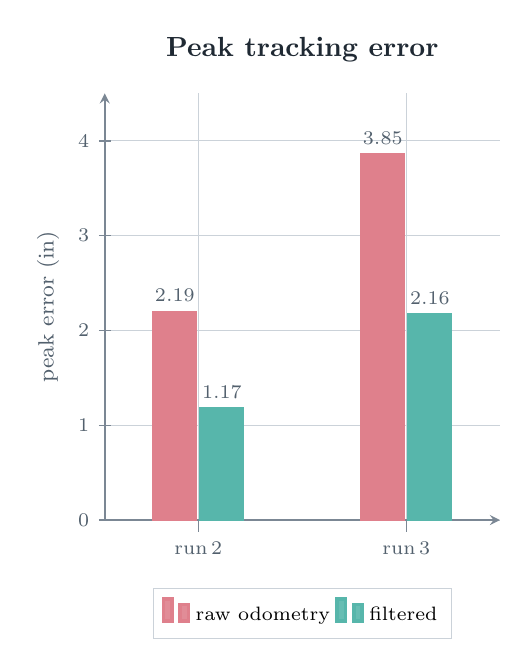
\begin{tikzpicture}
\begin{axis}[driftbase, width=6.6cm, height=7.0cm,
   title={Peak tracking error},
   ybar, bar width=15pt, ymin=0, ymax=4.5,
   symbolic x coords={run\,2, run\,3}, xtick=data,
   ylabel={peak error (in)}, enlarge x limits=0.45,
   nodes near coords, nodes near coords style={font=\scriptsize\color{subink}},
   legend style={font=\scriptsize, at={(0.5,-0.16)}, anchor=north, legend columns=2, draw=rulec}]
  \addplot[draw=drift!70, fill=drift!70] coordinates {(run\,2,\RunTwoRawMax) (run\,3,\RunThreeRawMax)};
  \addplot[draw=filt!75, fill=filt!75]   coordinates {(run\,2,\RunTwoNewMax) (run\,3,\RunThreeNewMax)};
  \legend{raw odometry, filtered}
\end{axis}
\end{tikzpicture}
\caption{Left: run\,3's south-west field quadrant (perimeter walls at
$-70.2$\,in, center structure top-right). The raw-odometry path bows away from the
filter's truth-anchored path as error accumulates around the cross. Right: peak
tracking error, raw vs.\ filtered --- roughly a \aggFactor$\times$ reduction on
both routes.}
\end{figure}

\subsection{What the two evidence runs say}
\begin{itemize}
  \item \textbf{Drift is real and directional.} Accepted fixes pointed almost
  entirely along one field axis --- run\,2's two fixes were $(0.10, 0.77)$ and
  $(0.02, 2.00)$\,in in $(x,y)$; run\,3's five ranged up to $(0.66, 3.72)$\,in ---
  consistent with a tank-drive scale/slip asymmetry, not random noise. Rate landed at
  \RunThreeDriftPer--\RunTwoDriftPer\,in per \SI{100}{in} travelled.
  \item \textbf{Continuous-only fusion trails the drift.} Capped at \contCap\,in per
  idle cycle, it returned a net \RunTwoNetApplied\,in (run\,2) and
  \RunThreeNetApplied\,in (run\,3) of the booked drift --- roughly half, always late.
  \item \textbf{The re-anchor closes the loop at the stop.} Peak modeled error falls
  \RunTwoRawMax$\to$\RunTwoNewMax\,in (run\,2) and
  \RunThreeRawMax$\to$\RunThreeNewMax\,in (run\,3); every segment then \emph{starts}
  from truth, which is what tightens run-to-run repeatability.
\end{itemize}


% ============================ GATES ========================================
\Needspace*{11cm}
\section{Why corrections are rare --- by design}
\begin{figure}[H]
\centering
\begin{tikzpicture}
\begin{axis}[driftbase, xbar, width=5.6cm, height=6.6cm,
   title={\footnotesize Run\,3: why scans were rejected},
   xlabel={MCL scans carrying each rejection flag (614 scans)},
   xmin=0, xmax=680, ytick=data, y dir=reverse,
   yticklabels from table={\rejecttable}{reason},
   yticklabel style={font=\tiny\ttfamily\color{subink}},
   bar width=6.5pt, enlarge y limits=0.07,
   nodes near coords, nodes near coords style={font=\tiny\color{subink}}]
  \addplot[draw=subink!70, fill=subink!35] table[x=count, y expr=\coordindex] {\rejecttable};
\end{axis}
\end{tikzpicture}\hfill
\begin{minipage}[b]{0.44\linewidth}
\scriptsize
\rowcolors{2}{panel}{white}
\begin{tabular}{c S[table-format=2.1] S[table-format=1.2] S[table-format=1.3] c c}
\toprule
\textbf{Run} & {\textbf{t (s)}} & {\textbf{$|$fix$|$ in}} & {\textbf{NIS}} &
\textbf{rays} & \textbf{inliers}\\
\midrule
\rawinput{data/accepts_rows.tex}
\bottomrule
\end{tabular}\\[4pt]
{\color{subink}All \nValidatedFixes{} accepted fixes. Flags overlap (a scan can fail
several gates at once); a fix lands only when \emph{every} gate passes. The
two-inlier rows are the robust local-range solve: the third ray was excluded as an
outlier (it saw a game object, not the wall) rather than being allowed to drag the
fix.}
\end{minipage}
\caption{Left: rejection-flag histogram over run\,3's 614 MCL scans --- motion
suppression dominates (the robot moves \RunThreeMotionPct\% of the time), then
geometry and stability gates. Right: the seven fixes that survived; accepted NIS sat
at \AcceptNisMin--\AcceptNisMax{} against a gate of 8.0 (4.0 for two-inlier
evidence).}
\end{figure}

% ============================ CHECKPOINTS ==================================
\section{Stop-by-stop accuracy against the commanded route}
At every stop of the tune routes the firmware records the commanded target
(\emph{Exp}) and the pose it believes it reached (\emph{Rep}); their difference
bundles PID settling, odometry drift, and applied corrections --- the practical
``how far off is the robot where it matters'' number. X/Y stayed within
\RunTwoCpMax\,in (run\,2) and \RunThreeCpMax\,in (run\,3) at every stop.

\begin{center}\scriptsize
\begin{minipage}[t]{0.46\linewidth}
\centering
{\footnotesize\bfseries\color{ink}Run\,2 --- square loop}\\[3pt]
\rowcolors{2}{panel}{white}
\begin{tabular}{c l S[table-format=+1.1] S[table-format=+1.1] S[table-format=+1.1] c}
\toprule
\# & \textbf{stop} & {$\Delta$x} & {$\Delta$y} & {$\Delta\theta\,^\circ$} & \textbf{rays}\\
\midrule
\rawinput{data/cp_run2_rows.tex}
\bottomrule
\end{tabular}
\end{minipage}\hfill
\begin{minipage}[t]{0.50\linewidth}
\centering
{\footnotesize\bfseries\color{ink}Run\,3 --- square $+$ cross}\\[3pt]
\rowcolors{2}{panel}{white}
\begin{tabular}{c l S[table-format=+2.1] S[table-format=+1.1] S[table-format=+2.1] c}
\toprule
\# & \textbf{stop} & {$\Delta$x} & {$\Delta$y} & {$\Delta\theta\,^\circ$} & \textbf{rays}\\
\midrule
\rawinput{data/cp_run3_rows.tex}
\bottomrule
\end{tabular}
\end{minipage}
\end{center}
\vspace{0.25em}
\noindent{\footnotesize\color{subink}Run\,3 stop 11's $+65.6^\circ$ is a turn that
hit its \SI{1200}{ms} timeout mid-rotation --- the next \texttt{moveToPose} absorbed
it (stop 12: $-0.8^\circ$). A motion-tuning datum, not a localization error. Heading
deltas right after turns ($\approx$$-5^\circ$) are PID settle/timeout, visible
because capture happens immediately at motion end; they relax by the next stop. The
May~24 pre-calibration sweep (\texttt{tune.txt}) showed a constant
\TuneSweepBias$^\circ$ bias at \emph{every} commanded angle --- the signature that
fed the sensor-angle calibration now in \texttt{localization\_config.cpp}.}

% ============================ TABLE ========================================
\Needspace*{7cm}
\section{All seven runs}
\begin{center}\footnotesize
\rowcolors{2}{panel}{white}
\begin{tabular}{l l S[table-format=4.0] S[table-format=2.1] S[table-format=3.0]
   S[table-format=2.0] S[table-format=1.0] c c c}
\toprule
\textbf{Run} & \textbf{Route / condition} & {\textbf{rows}} & {\textbf{s}} & {\textbf{path,in}} &
{\textbf{mot\%}} & {\textbf{fixes}} & {\textbf{booked,in}} & {\textbf{filt,in}} & \textbf{gain}\\
\midrule
1 & sample route (pre-guard)    & \RunOneRows   & \RunOneDur   & \RunOnePath   & \RunOneMotionPct   & \RunOneAccepts   & {---} & {---} & {---}\\
2 & square loop                 & \RunTwoRows   & \RunTwoDur   & \RunTwoPath   & \RunTwoMotionPct   & \RunTwoAccepts   & \RunTwoRawMax   & \RunTwoNewMax   & \textbf{\RunTwoFactor$\times$}\\
3 & square $+$ cross            & \RunThreeRows & \RunThreeDur & \RunThreePath & \RunThreeMotionPct & \RunThreeAccepts & \RunThreeRawMax & \RunThreeNewMax & \textbf{\RunThreeFactor$\times$}\\
4 & sample route, blocked view  & \RunFourRows  & \RunFourDur  & \RunFourPath  & \RunFourMotionPct  & \RunFourAccepts  & {---} & {---} & {---}\\
5 & forced weak start (pre-guard) & \RunFiveRows & \RunFiveDur & \RunFivePath  & \RunFiveMotionPct  & \RunFiveAccepts  & {---} & {---} & {---}\\
6 & weak start, guard active    & \RunSixRows   & \RunSixDur   & \RunSixPath   & \RunSixMotionPct   & \RunSixAccepts   & {---} & {---} & {---}\\
7 & clean start, guard active   & \RunSevenRows & \RunSevenDur & \RunSevenPath & \RunSevenMotionPct & \RunSevenAccepts & {---} & {---} & {---}\\
\bottomrule
\end{tabular}
\end{center}
\noindent{\footnotesize\color{subink}\textbf{booked}/\textbf{filt} are the modeled
peak position errors (sensor-booked raw drift vs.\ boundary re-anchor replay);
\textbf{fixes} counts validated accept events. Runs 1 and 4--7 produced no
mid-route fix (blocked or weak sensor views, or near-continuous motion at
\numrange{86}{88}\%), so the filter correctly returned raw odometry --- a dash means
``no drift was bookable,'' not ``no drift.'' Provenance: runs 1 and 4 predate the
build that stamps \texttt{test\_case} into the header; their stale ``Turn center''
label is cosmetic (route identified by path length and absent checkpoints --- see
\texttt{validation\_data/README.txt}).}

% ============================ GOALS ========================================
\section{Against the three goals}
\subsection{\faBullseye\; Accuracy}
The filter does not invent accuracy --- it imports it from the walls. At the start it
fixes the absolute pose to the wall solver's agreement envelope (reproduced to
\AuditWallMaxErr\,in); mid-route, when the sensors get a clean look (runs 2--3), it
removes \numrange{1}{4}\,in of real, directional odometry error. When they do not,
there is nothing trustworthy to add, and it says so by staying on odometry.

\subsection{\faSync\; Repeatability}
The structural win. Raw odometry's end pose inherits the variance of \emph{every}
slip since the start; the re-anchor zeroes that integral at each validated stop, so
the end pose inherits only the \emph{last} segment's drift. Run\,3 shows it
directly: a fix at the final stop brings the modeled end error to
\RunThreeNewEnd\,in versus \RunThreeRawEnd\,in for raw odometry. And because the
start relocalizes, that repeatability is anchored to the \emph{field}, not to
wherever the robot happened to be placed.

\subsection{\faBolt\; Speed}
No cost. Corrections are structurally forbidden while a motion runs (the dominant
bar in the rejection histogram), so the controller never chases a moving pose. The
re-anchor fires only in the idle beat between segments. Driving speed is untouched;
only the \emph{reference} each segment starts from gets better.

% ============================ AUDIT ========================================
\section{Audit: does the firmware do what the math says?}\label{sec:audit}
This pass re-derived every number above from the raw logs with an independent
reimplementation of the geometry, and checked the code's invariants against what the
robot actually recorded.

\begin{center}\footnotesize
\begin{tabular}{l l l}
\toprule
\textbf{Invariant checked} & \textbf{Result} & \\
\midrule
Ray-cast sensor model (walls $+$ obstacle), replayed offline & max
  $\Delta$ \AuditRayMaxErr\,in over \AuditRayCount{} predictions & \ok\\
Wall-solve commits, re-derived from raw snapshots & max $\Delta$
  \AuditWallMaxErr\,in across all six commits & \ok\\
Divergence is a pure staircase (steps only at accepts) & max off-accept step
  \AuditStairMax\,in & \ok\\
Correction limiter honors its cap & max applied step \AuditCapObserved\,in
  $\leq$ \AuditCapBound\,in bound & \ok\\
Motion suppression / accept gating consistent with flags & all
  \nValidatedFixes{} accepts fully gated; zero while suppressed & \ok\\
Odometry delta stream continuity & no mid-route sequence gaps in any run & \ok\\
\bottomrule
\end{tabular}
\end{center}

\subsection{Fixed in this audit pass}
\begin{itemize}
  \item \textbf{Field-frame heading prior.} Relocalization read the \emph{raw} IMU
  rotation as its heading prior --- correct only because the current routine starts
  at heading $0^\circ$. It now uses the odometry heading (IMU-driven, but expressed
  in the field frame), so any future start heading works unchanged.
  \item \textbf{Walls no longer vote on heading.} The wall solver previously swept
  four snapped cardinals and committed the winner's cardinal as the robot's heading
  --- on a near-square field, an alias trap held shut only by an IMU gate in the
  wrong reference frame. It now solves once, at the trusted heading; X/Y comes from
  the walls, heading stays IMU-true. (Identical behavior on all seven validation
  runs, by construction.)
  \item \textbf{One-shot hygiene.} A pending boundary re-anchor request could
  survive a localization stop/start cycle; it is now cleared on start.
  \item \textbf{Single source of truth.} A retired copy of the relocalization
  machinery (including the old two-sensor accept rule that produced run\,5's false
  commit) still lived in the tune harness --- 360 lines of dead logic, deleted.
\end{itemize}

% ============================ CAVEATS ======================================
\section{What this does and does not prove}
\begin{tcolorbox}[enhanced, colback=paneldrift, colframe=drift!55, boxrule=0.7pt,
  arc=3pt, left=9pt, right=9pt, top=7pt, bottom=7pt]
\begin{itemize}[leftmargin=1.3em]
  \item \textbf{Truth is the gated filter, not a tape measure.} Absolute drift
  figures are conservative \emph{lower bounds} (only sensor-booked drift counts);
  the improvement ratio is geometric and robust to that. The tape-measure protocol
  that closes this is written and pending: \texttt{validation\_data/field\_test\_protocol.md}.
  \item \textbf{The re-anchor and the audited relocalization changes have not yet
  run on hardware.} These traces predate both: the re-anchor curves are the
  validated fixes replayed at the stops, and the heading-prior fix is
  behavior-identical on these runs by construction. Protocol tests 2--3 confirm them
  on the robot.
  \item \textbf{The gain is route- and geometry-limited.} Two routes yielded
  \numrange{2}{5} fixes because the robot moves \numrange{86}{95}\% of the time.
  More and better-placed wall views raise the factor; that is tuning
  (sensor placement, stop placement), not logic.
  \item \textbf{Heading accuracy is not claimed.} Ranges never steer heading by
  design; all error figures are X/Y position.
\end{itemize}
\end{tcolorbox}

\vspace{0.5em}
\noindent{\small\color{subink}\faSync\; \textbf{Reproduce:} \texttt{python3
tools/drift\_analysis.py \&\& python3 tools/audit\_analysis.py} regenerates every
number, table row, and data file; then \texttt{latexmk -pdf} on this document.}

\end{document}
